\documentclass[list,mac]{BHCexam}
\pagestyle{fancy}
\fancyfoot[C]{\kaishu \small 第 \thepage 页 共 \pageref{lastpage} 页}
%\fancyhead[L]{
\includegraphics[width=2cm]{qrcode.png}}
\begin{document}
\title{2019年浙江高考}
\subtitle{数学试卷}
\maketitle
\noindent\textbf{注意事项:} \\
\noindent\text{1.答题前,考生先将自己的姓名、准考证号码填写清楚,将条形码准确粘贴在条形码区域内;}\\
\noindent\text{2.选择题必须使用2B铅笔填土,非选择题必须使用0.5毫米黑色字迹的签字笔书写;}\\
\noindent\text{3.请按照题号顺序在答题卡的答题区域内作答,超出答题区域的其他地方答案无效;}\\
\noindent\text{4.作图可先试用铅笔画出,确定后必须用黑色签字笔描黑;}\\
\noindent\text{5.保持卡面清洁、不要折叠、弄破,不准使用修正带、涂改液、刮纸刀.}\\
\begin{groups}

\group{选择题}{本大题共10小题,共50.0分}

\begin{questions}[30s]
\question[6]行驶中的汽车如果发生剧烈碰撞,车内的安全气囊会被弹出并瞬间充满气体.若碰撞后汽车的速度在很短时间内减小为零,关于安全气囊在此过程中的作用,下列说法正确的是\key{D}
\fourchoices{增加了司机单位面积的受力大小}{减少了碰撞前后司机动量的变化量}{将司机的动能全部转换成汽车的动能}{延长了司机的受力时间并增大了司机的受力面积}
\begin{solution}{4cm}

\end{solution}



\question[6]火星的质量约为地球质量的$1/10,$半径约为地球半径的$1/2,$则同一物体在火星表面与在地球表面受到的引力的比值约为\key{B}
\fourchoices{$0.2$}{$0.4$}{$2.0$}{$2.5$}
\begin{solution}{4cm}

\end{solution}



\question[6]如图,一同学表演荡秋千.已知秋千的两根绳长均为$10m,$该同学和秋千踏板的总质量约为$50kg.$绳的质量忽略不计,当该同学荡到秋千支架的正下方时,速度大小为$8m/s,$此时每根绳子平均承受的拉力约为\key{B}
\begin{center}
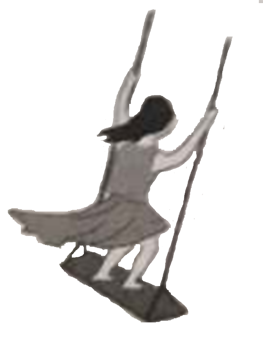
\includegraphics[]{img/image1.png}
\end{center}

\fourchoices{$200N$}{$400N$}{$600N$}{$800N$}
\begin{solution}{4cm}

\end{solution}


\newpage
\question[6]图(a)所示的电路中,K与L间接一智能电源,用以控制电容器C两端的电压$U_C.$如果$U_C$随时间t的变化如图(b)所示,则下列描述电阻R两端电压$U_R$随时间t变化的图像中,正确的是\key{A}
\begin{center}
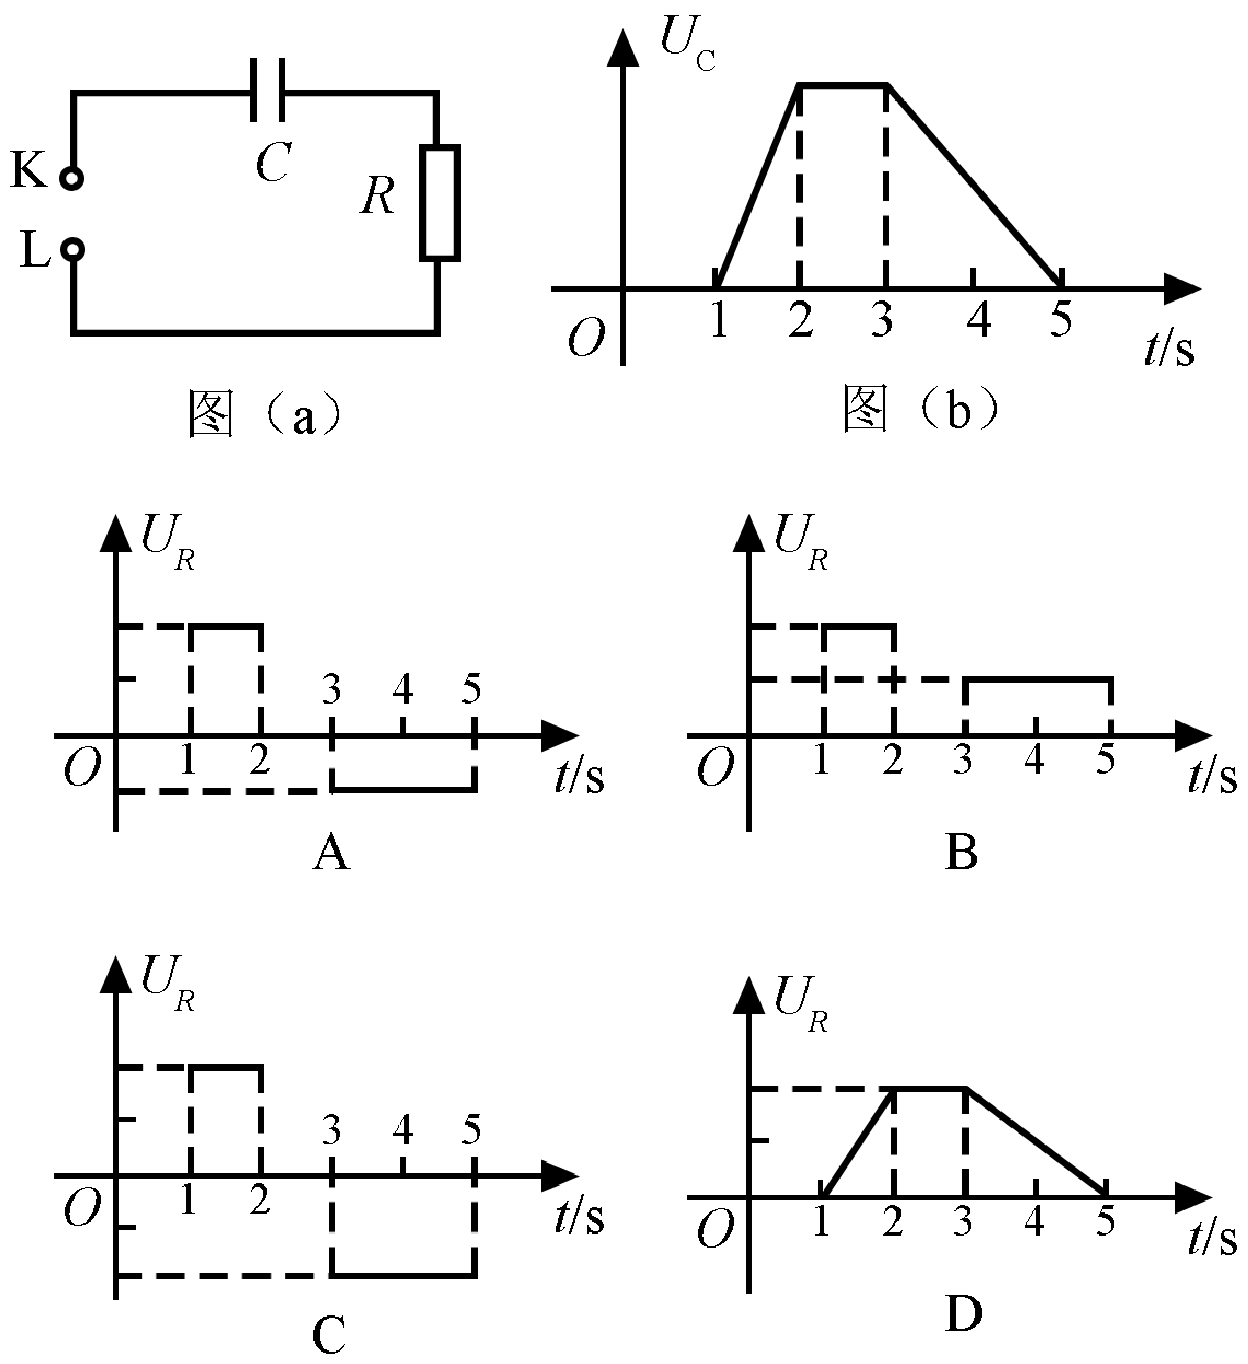
\includegraphics[width=8cm]{img/image2.png}
\end{center}
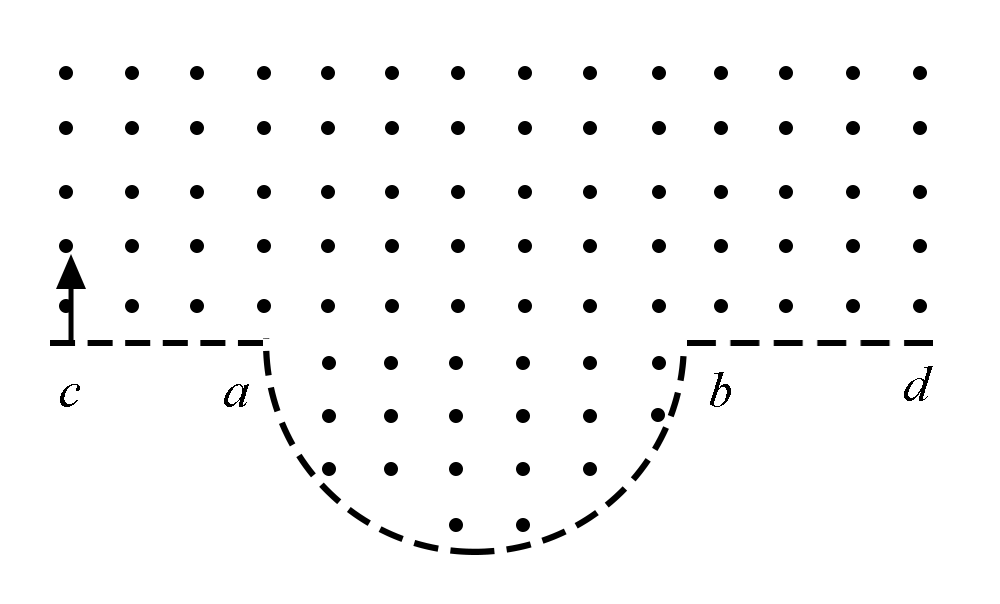
\includegraphics[width=3.5cm]{img/image3.png}
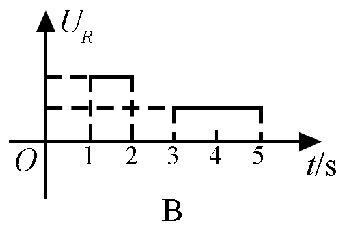
\includegraphics[width=3.5cm]{img/image4.png}
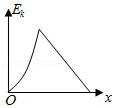
\includegraphics[width=3.5cm]{img/image5.png}
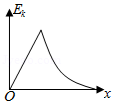
\includegraphics[width=3.5cm]{img/image6.png}

\begin{solution}{4cm}

\end{solution}



\question[6]一匀强磁场的磁感应强度大小为B,方向垂直于纸面向外,其边界如图中虚线所示$,ab$为半圆$,ac、bd$与直径ab共线$,ac$间的距离等于半圆的半径.一束质量为m、电荷量为$q(q>0)$的粒子,在纸面内从c点垂直于ac射入磁场,这些粒子具有各种速率.不计粒子之间的相互作用.在磁场中运动时间最长的粒子,其运动时间为\key{C}
\begin{center}
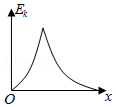
\includegraphics[]{img/image7.png}
\end{center}

\fourchoices{$\frac{7\pi m}{6qB}$}{$\frac{5\pi m}{4qB}$}{$\frac{4\pi m}{3qB}$}{$\frac{3\pi m}{2qB}$}
\begin{solution}{4cm}

\end{solution}



\question[6]下列核反应方程中$,X_1,X_2,X_3,X_4$代表α粒子的有\key{BD}
\fourchoices{$_1^2H+_1^2H→_0^10^n+X_1$}{$^{2}_{1}H+_{1}^{3}H\rightarrow_{0}^{1}n+X_{2}$}{$_{92}^{235}U+_{0}^{1}n\rightarrow_{56}^{144}Ba+\frac{89}{36}Kr+3X_{3}$}{$_{0}^{1}n+\frac{6}{3}Li\rightarrow_{1}^{3}H+X_{4}$}
\begin{solution}{4cm}

\end{solution}


\newpage
\question[6]一物块在高$3.0m$、长$5.0m$的斜面顶端从静止开始沿斜面下滑,其重力势能和动能随下滑距离s的变化如图中直线\uppercase\expandafter{\romannumeral1}、\uppercase\expandafter{\romannumeral2 }所示,重力加速度取$10m/s^2.$则\key{AB}
\begin{center}
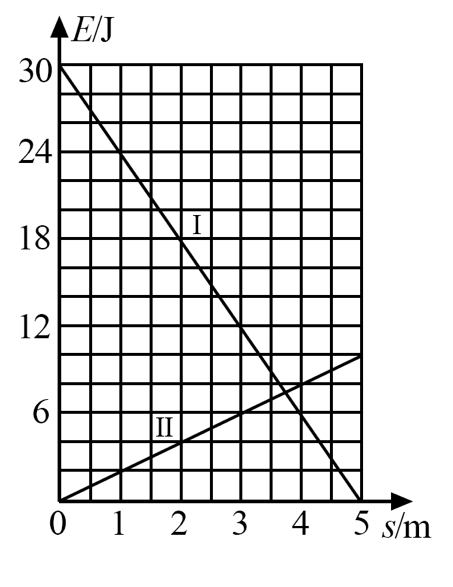
\includegraphics[]{img/image8.png}
\end{center}

\fourchoices{物块下滑过程中机械能不守恒}{物块与斜面间的动摩擦因数为$0.5$}{物块下滑时加速度的大小为$6.0m/s^2$}{当物块下滑$2.0m$时机械能损失了$12J$}
\begin{solution}{4cm}

\end{solution}



\question[6]如图,U形光滑金属框$abcd$置于水平绝缘平台上$,ab$和dc边平行,和bc边垂直$.ab$、$dc$足够长,整个金属框电阻可忽略.一根具有一定电阻的导体棒MN置于金属框上,用水平恒力F向右拉动金属框,运动过程中,装置始终处于竖直向下的匀强磁场中$,MN$与金属框保持良好接触,且与bc边保持平行.经过一段时间后\key{BC}
\begin{center}
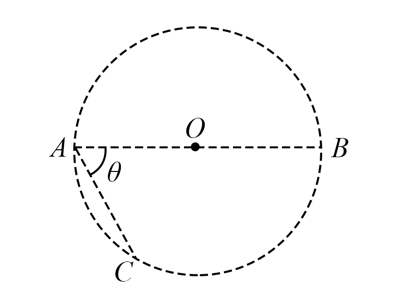
\includegraphics[]{img/image9.png}
\end{center}

\fourchoices{属框的速度大小趋于恒定值}{属框的加速度大小趋于恒定值}{体棒所受安培力的大小趋于恒定值}{体棒到金属框bc边的距离趋于恒定值}
\begin{solution}{4cm}

\end{solution}
\newpage



\end{questions}

\group{填空题}{本大题共7小题,共36.0分}

\begin{questions}[p]
\question[4] 复数$z= \dfrac {1}{1+i} (i$为虚数单位$)$,则$|z|=$\key{$ \dfrac { \sqrt {2}}{2}$}.
\begin{solution}{4cm}

\end{solution}



\question[6] 已知圆$C$的圆心坐标是$(0 , m)$,半径长是$r.$若直线$2x-y+3=0$与圆$C$相切于点$A(-2 , -1)$,则$m=$\key{$-2$  $ \sqrt {5}$  },$r=$
\begin{solution}{4cm}

\end{solution}



\question[6] 在二项式$( \sqrt {2} +x) ^{9}$展开式中,常数项和系数为有理数的项的个数分别是\key{$16 \sqrt {2}$ , $5$  }
\begin{solution}{4cm}

\end{solution}



\question[6] 在$\triangle ABC$中,$ \angle ABC=90^{\small \circ}$,$AB=4$,$BC=3$,点$D$在线段$AC$上,若$ \angle BDC=45^{\small \circ}$,则$BD=$\key{$ \dfrac {12 \sqrt {2}}{5}$  $ \dfrac {7 \sqrt {2}}{10}$  },$\cos \angle ABD=$
\begin{solution}{4cm}

\end{solution}



\question[4] 已知椭圆$ \dfrac {x^{2}}{9} + \dfrac {y^{2}}{5} =1$的左焦点为$F$,点$P$在椭圆上且在$x$轴的上方$.$若线段$PF$的中点在以原点$O$为圆心,$|OF|$为半径的圆上,则直线$PF$的斜率是\key{$ \sqrt {15}$}.
\begin{solution}{4cm}

\end{solution}



\question[4] 已知$a \in \mathbf R$,函数$f(x)=ax ^{3} -x.$若存在$t \in \mathbf R$,使得$|f(t+2)-f(t)|\leqslant \dfrac {2}{3}$,则实数$a$的最大值是\key{$ \dfrac {4}{3}$}.
\begin{solution}{4cm}

\end{solution}



\question[6] 已知正方形$ABCD$的边长为$1.$当每个$ \lambda  _{i} (i=1 , 2 , 3 , 4 , 5 , 6)$取遍$ \pm 1$时,$| \lambda  _{1} \overrightarrow{AB} + \lambda  _{2} \overrightarrow{BC} + \lambda  _{3} \overrightarrow{CD} + \lambda  _{4} \overrightarrow{DA} + \lambda  _{5} \overrightarrow{AC} + \lambda  _{6} \overrightarrow{BD} |$的最小值是\key{$0$},最大值是\key{$2 \sqrt {5}$}.
\begin{solution}{4cm}

\end{solution}

\end{questions}

\group{解答题}{本大题共5小题,共71.0分}

\begin{questions}[p]

\question[14] 设函数$f(x)=sinx$,$x \in R$.
\begin{subquestions}
    \subquestion $($\Romannum{1}$)$已知$ \theta  \in [0 , 2 \pi )$,函数$f(x+ \theta )$是偶函数,求$ \theta $的值;
    \subquestion $($\Romannum{2}$)$求函数$y=[f(x+ \dfrac { \pi }{12} )] ^{2} +[f(x+ \dfrac { \pi }{4} )] ^{2}$的值域.
\end{subquestions}
\begin{solution}{6cm}

\end{solution}



\question[15] 如图,已知三棱柱$ABC-A _{1} B _{1} C _{1}$,平面$A _{1} ACC _{1}  \perp $平面$ABC$,$ \angle ABC=90^{\small \circ}$,$ \angle BAC=30^{\small \circ}$,$A _{1} A=A _{1} C=AC$,$E$,$F$分别是$AC$,$A _{1} B _{1}$的中点.
\begin{subquestions}
    \subquestion $($\Romannum{1}$)$证明:$EF \perp BC$;
    \subquestion $($\Romannum{2}$)$求直线$EF$与平面$A _{1} BC$所成角的余弦值.
\end{subquestions}

\begin{solution}{6cm}

\end{solution}



\question[15] 设等差数列$\{a _{n} \}$的前$n$项和为$S _{n}$,$a _{3} =4$,$a _{4} =S _{3} .$数列$\{b _{n} \}$满足:对每个$n \in N ^{*}$,$S _{n} +b _{n}$,$S _{n+1} +b _{n}$,$S _{n+2} +b _{n}$成等比数列.
\begin{subquestions}
    \subquestion $($\Romannum{1}$)$求数列$\{a _{n} \}$,$\{b _{n} \}$的通项公式;
    \subquestion $($\Romannum{2}$)$记$c _{n} = \sqrt { \dfrac {a_{n}}{2b_{n}}}$,$n \in N ^{*}$,证明:$c _{1} +c _{2} + \cdots +c _{n}  \lt  2 \sqrt {n}$,$n \in N ^{*}$.
\end{subquestions}
\begin{solution}{6cm}

\end{solution}



\question[12] 如图,已知点$F(1 , 0)$为抛物线$y ^{2} =2px(p  \gt  0)$的焦点$.$过点$F$的直线交抛物线于$A$,$B$两点,点$C$在抛物线上,使得$\triangle ABC$的重心$G$在$x$轴上,直线$AC$交$x$轴于点$Q$,且$Q$在点$F$的右侧$.$记$\triangle AFG$,$\triangle CQG$的面积分别为$S _{1}$,$S _{2}$.
\begin{subquestions}
    \subquestion 求$p$的值及抛物线的准线方程;
    \subquestion 求$ \dfrac {S_{1}}{S_{2}}$的最小值及此时点$G$点坐标.
\end{subquestions}

\begin{solution}{6cm}

\end{solution}
\question[15] 已知实数$a\neq 0$,设函数$f(x)=a\ln x+ \sqrt {1+x}$,$x  \gt  0$.
\begin{subquestions}
    \subquestion $($\Romannum{1}$)$当$a=- \dfrac {3}{4}$时,求函数$f(x)$的单调区间;
    \subquestion $($\Romannum{2}$)$对任意$x \in \Big[ \dfrac {1}{\mathrm e^{2}} , + \infty \Big)$均有$f(x)\leqslant \dfrac { \sqrt {x}}{2a}$,求$a$的取值范围.
    \subquestion 注意:$\mathrm e=2.71828 \cdots  \cdots $为自然对数的底数.
\end{subquestions}
\begin{solution}{6cm}

\end{solution}




\end{questions}
\end{groups}
\label{lastpage}
\end{document}
